\documentclass{beamer}
\usetheme{Madrid}

\usepackage{amsmath, amssymb, amsthm}
\usepackage{graphicx}
\usepackage{listings}
\usepackage{gensymb}
\usepackage[utf8]{inputenc}
\usepackage{hyperref}
\usepackage{gvv}
\usepackage{gensymb}

\begin{document}

\title{MATGEO: 7-7.2-19}
\author{AI24BTECH11020 - Rishika Kotha$^{}$% <-this % stops a space
}
\frame{\titlepage}

\begin{frame}
\frametitle{Question}
Equation of the circle with centre on the Y axis and passing through the origin and the point (2, 3) is
 \\
\begin{enumerate}
    a. $3x^2+3y^2-13y=0$
    b. $3x^2+3y^2+13x+3=0$
    c. $6x^2+6y^2-13x=0$
    d. $x^2+y^2+13x+3=0$
\end{enumerate} \hfill(MATGEO 7-7.2-19)
\end{frame}


\begin{frame}{allowframebreaks}
\frametitle{Solution: Theory}
        \begin{table}[h!]
    \centering
    \begin{tabular}[12pt]{ |c| c| c|}
    \hline
	parameter & Description & value \\ 
    \hline
	 C & Centre & $\myvec{0\\ 13/6}$\\
    \hline 
	 O & point1 & $\myvec{0\\0}$\\
    \hline
	 P & point2 & $\myvec{2\\3}$\\
    \hline   
	 r & radius & 13/6\\
    \hline
    \end{tabular}

    \label{7-7.2-19}
        \end{table}
\end{frame}

\begin{frame}{allowframebreaks}
\frametitle{Given Data}
From the given information,
\begin{align}
	x_1=\myvec{2\\3}, x_2=\myvec{0\\0},n=\myvec{1\\0},c=0 
\end{align}
\begin{align}
    \myvec{4 & 6 & 1 \\
               0 & 0 & 1 \\
               -1 & 0 & 0}
               \myvec{u\\f}=\myvec{-13\\0\\0}
\end{align}
The augmented matrix is expressed as
	\begin{align}
        \myvec{4 & 6 & 1 & \vrule & -13\\
         0 &  0 & 1 & \vrule & 0\\                                                 
         -1 &  0 & 0 & \vrule & 0}       
\end{align}
\end{frame}
\begin{frame}{allowframebreaks}
\frametitle{Row Operations}
performing sequences of row operations to transform into Echelon form
\begin{align}
	\underleftrightarrow{R_3 \rightarrow 4R_3+R_1}
         \myvec{4 & 6 & 1 & \vrule & -13\\
         0 &  0 & 1 & \vrule & 0\\
         0 &  6 & 1 & \vrule & -13}
         \underleftrightarrow{R_1\rightarrow R_1-R_3}
         \myvec{4 & 0 & 0 & \vrule & 0\\
         0 & 0 & 1 & \vrule & 0\\
         0 & 6 & 1 &\vrule & -13}\\
         \underleftrightarrow{R_2\rightarrow R_2-R_3}
         \myvec{4 & 0 & 0 &\vrule & 0\\
         0 & -6 & 0 & \vrule & 13 \\
         0 & 6 & 1 & \vrule & -13}
         \underleftrightarrow{R_3\rightarrow R_3+R_2}
         \myvec{4 & 0 & 0 &\vrule & 0\\
         0 & -6 & 0 & \vrule & 13 \\
         0 & 0 & 1 & \vrule & 0}\\
         \underleftrightarrow{R_1\rightarrow R_1/4, R_2 \rightarrow R_2/-6}
\myvec{1 & 0 & 0 &\vrule & 0\\
         0 & 1 & 0 & \vrule & -13/6 \\
         0 & 0 & 1 & \vrule & 0} 
\end{align}
\begin{align}
   u=\myvec{0 \\ -13/6},f=0
\end{align}
$\therefore$ the equation of the circle is $3x^2+3y^2-13y=0$.
\end{frame}


\begin{frame}{allowframebreaks}
\frametitle{Graph}
\begin{figure}[ht]
\centering
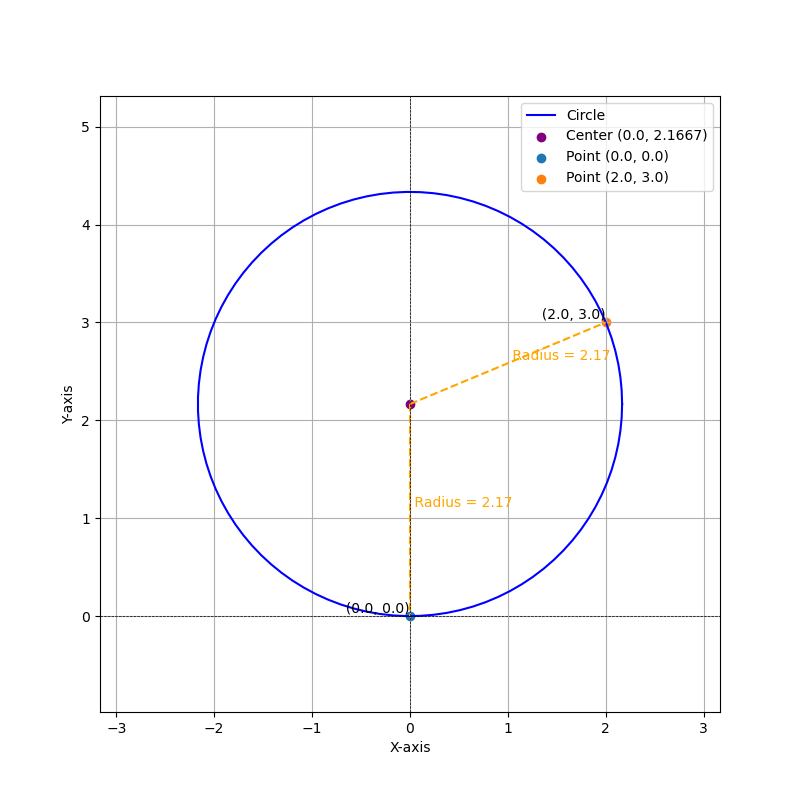
\includegraphics[width=0.7\linewidth]{figs/Fig1.png}
\end{figure}
\end{frame}


\begin{frame}{allowframebreaks}
\frametitle{C-Code}
#include <stdio.h>
int main() {
    float centerX = 0.0f, centerY = 2.1667f; 
    float radius = 2.1667f;                    
    float points[2][2] = { {0.0f, 0.0f}, {2.0f, 3.0f} }; 
    float *center = &centerX;
    float *radiusPtr = &radius;
    float (*pointsPtr)[2] = points; 
    FILE *file = fopen("data.txt", "w");
    if (file == NULL) {
        perror("Error opening file");
        return 1;}
    fprintf(file, "Center: %.4f, %.4f\n", *center, *(center + 1));
    fprintf(file, "Radius: %.4f\n", *radiusPtr);
    fprintf(file, "Points: (%.1f, %.1f), (%.1f, %.1f)\n", 
            pointsPtr[0][0], pointsPtr[0][1], pointsPtr[1][0], pointsPtr[1][1]);
    fclose(file);
    printf("Data written to data.txt successfully.\n");
    return 0;
}

\end{frame}


\begin{frame}{allowframebreaks}
\frametitle{Python-Code}
import numpy as np
import matplotlib.pyplot as plt
def read_data(file_name):
    with open(file_name, 'r') as file:
        lines = file.readlines()
    center = tuple(map(float, lines[0].strip().split(':')[1].strip().split(',')))
    radius = float(lines[1].strip().split(':')[1].strip())
    points_line = lines[2].strip().split(':')[1].strip()
    points = [tuple(map(float, p.strip().strip('()').split(','))) for p in points_line.split('), (')]
    return center, radius, points
center, radius, points = read_data('data.txt')
theta = np.linspace(0, 2 * np.pi, 100)
x_circle = radius * np.cos(theta) + center[0]
y_circle = radius * np.sin(theta) + center[1]
plt.figure(figsize=(8, 8))
plt.plot(x_circle, y_circle, label='Circle', color='blue')
plt.scatter(center[0], center[1], color='purple', label=f'Center {center}')
for point in points:
    plt.scatter(*point, label=f'Point {point}')
for point in points:
    plt.plot([center[0], point[0]], [center[1], point[1]], color='orange', linestyle='--')
    mid_x = (center[0] + point[0]) / 2
    mid_y = (center[1] + point[1]) / 2
    plt.text(mid_x, mid_y, f' Radius = {radius:.2f}', fontsize=10, color='orange', verticalalignment='bottom')
for point in points:
    plt.text(point[0], point[1], f'  {point}', fontsize=10, verticalalignment='bottom', horizontalalignment='right')
plt.axis('equal')
plt.xlim(center[0] - radius - 1, center[0] + radius + 1)
plt.ylim(center[1] - radius - 1, center[1] + radius + 1)
plt.axhline(0, color='black', linewidth=0.5, ls='--')
plt.axvline(0, color='black', linewidth=0.5, ls='--')
plt.xlabel('X-axis')
plt.ylabel('Y-axis')
plt.lege
\end{frame}

\end{document}
